\documentclass[11pt,a4paper]{article}

\usepackage{jheppub}
\usepackage{dsfont}
\usepackage{nicefrac}
\usepackage{bm}
\usepackage{mathsettings}
\usepackage{xparse}
\usepackage{mathrsfs}
\usepackage[none]{hyphenat}
\usepackage{tabularx}
\usepackage{makecell}
\usepackage{empheq}
\usepackage{pifont}

\newcommand{\bfnt}[1]{{\bfseries #1}}
\newcommand{\ifnt}[1]{{\itshape #1}}

% https://tex.stackexchange.com/a/531829/200495
\makeatletter
\gdef\@fpheader{}
\makeatother


\begin{document}

	\title{A Brief Primer on X-ray Diffraction Crystallography}
	\author{Wrichik Basu}
	\affiliation{Dept. of Physics, Scottish Church College, University of Calcutta}
	\date{\today}
	
	\maketitle
	
	\section{Introduction}
	
	\section{Spectroscopy vs. Crystallography}
	
		\textbf{Spectroscopy} is the study of absorption and/or emission of electromagnetic radiation in which the incident radiation interacts with the molecule and produces characteristic signals. From spectroscopy, we can get the following data about a molecule: %
%			
			\begin{itemize}%
%		
			    \item Bond lengths and bond angles of simple (diatomic, triatomic) molecules.
			    
			    \item Combination of Infrared and NMR (${}^1 \mathrm{H}$ and ${}^{13} \mathrm{C}$) spectroscopy provides information about functional groups, bond connectivity and stereochemistry (absolute configuration) of simple molecules.
		    
		    \end{itemize}
		    
		Spectroscopy, however, cannot provide information about bond lengths, bond angles, torsion angles, etc. of complicated molecules.
		
		\textbf{Crystallography}, on the other hand, deals in the interaction of EM radiation of very small wavelength ($\lambda \sim \SI{1}{\angstrom}$) with solid materials (crystalline or amorphous) through scattering. The main difference with spectroscopy is that in crystallography, there is no absorption ot emission of radiation; only scattering of radiation. Crystallography allows us to study%
%			
			\begin{itemize}%
%			
			    \item Accurate bond length, bond angles, torsion angles, precise absolute configuration, etc. of all types of crystalline substances.
			    
			    \item 3D structure of crystalline substances can lead to intermolecular or interionic interactions. Structure property relationship can be obtained using data from crystallography.
			    
			\end{itemize}
			
	\section{Why X-rays?}
	
		
	\section{Sources of X-rays}

	For X-ray diffraction experiments, monochromatic radiation from various metal-based sources (eg. Cu, Ag, Mo) is used in the lab. There are also synchotron-based sources for X-rays.%
%			
	\begin{itemize}%
%			
	    \item \bfnt{Sealed-tube X-ray sources}%
%			    	
	    	\begin{itemize}[label={$\hookrightarrow$}]%
%			    	
	    	    \item \ul{Fine focus sources}: Operate at around $50~\si{kV}$ and $40~\si{mA}$ ($\sim \SI{2}{kW}$). Can give a photon flux of around $\SI{1e7}{photons/s~mm^2}.$
	    	    
	    	    \item \ul{Microfocus sources}: Highly focussed beam. Operates at $40-50~\si{kV}$ and $2-15~\si{mA}$  ($<\SI{1}{kW}$). Can provide around $\SI{1e8}{photons/s~mm^2}.$
	    	    
	    	\end{itemize}
	    	
	    \item \bfnt{Rotating anode based source}: The anode is rotated at a very high speed of around $10,000~\si{rpm}.$ Cu, Mo or dual anode is used. Generally microfocus-based system. Operates at $\SI{60}{kV}$ and $\SI{100}{mA}$ or higher ($> \SI{6}{kW}$). Can produce a flux $\sim \num{1e10}-\num{e11}~\si{photons/s~mm^2}.$
	    
	    \item \bfnt{Metal Jet source}: Liquid Gallium is used, giving $\lambda = \SI{1.340}{\angstrom}.$ High intensity at much low power. Can generate $\sim \num{1e11}-\num{e12}~\si{photons/s~mm^2}.$
	    
	    \item Synchotron Sources:
	    
	\end{itemize}
	
	\section{Generating X-rays}

\begin{figure}
	\centering
	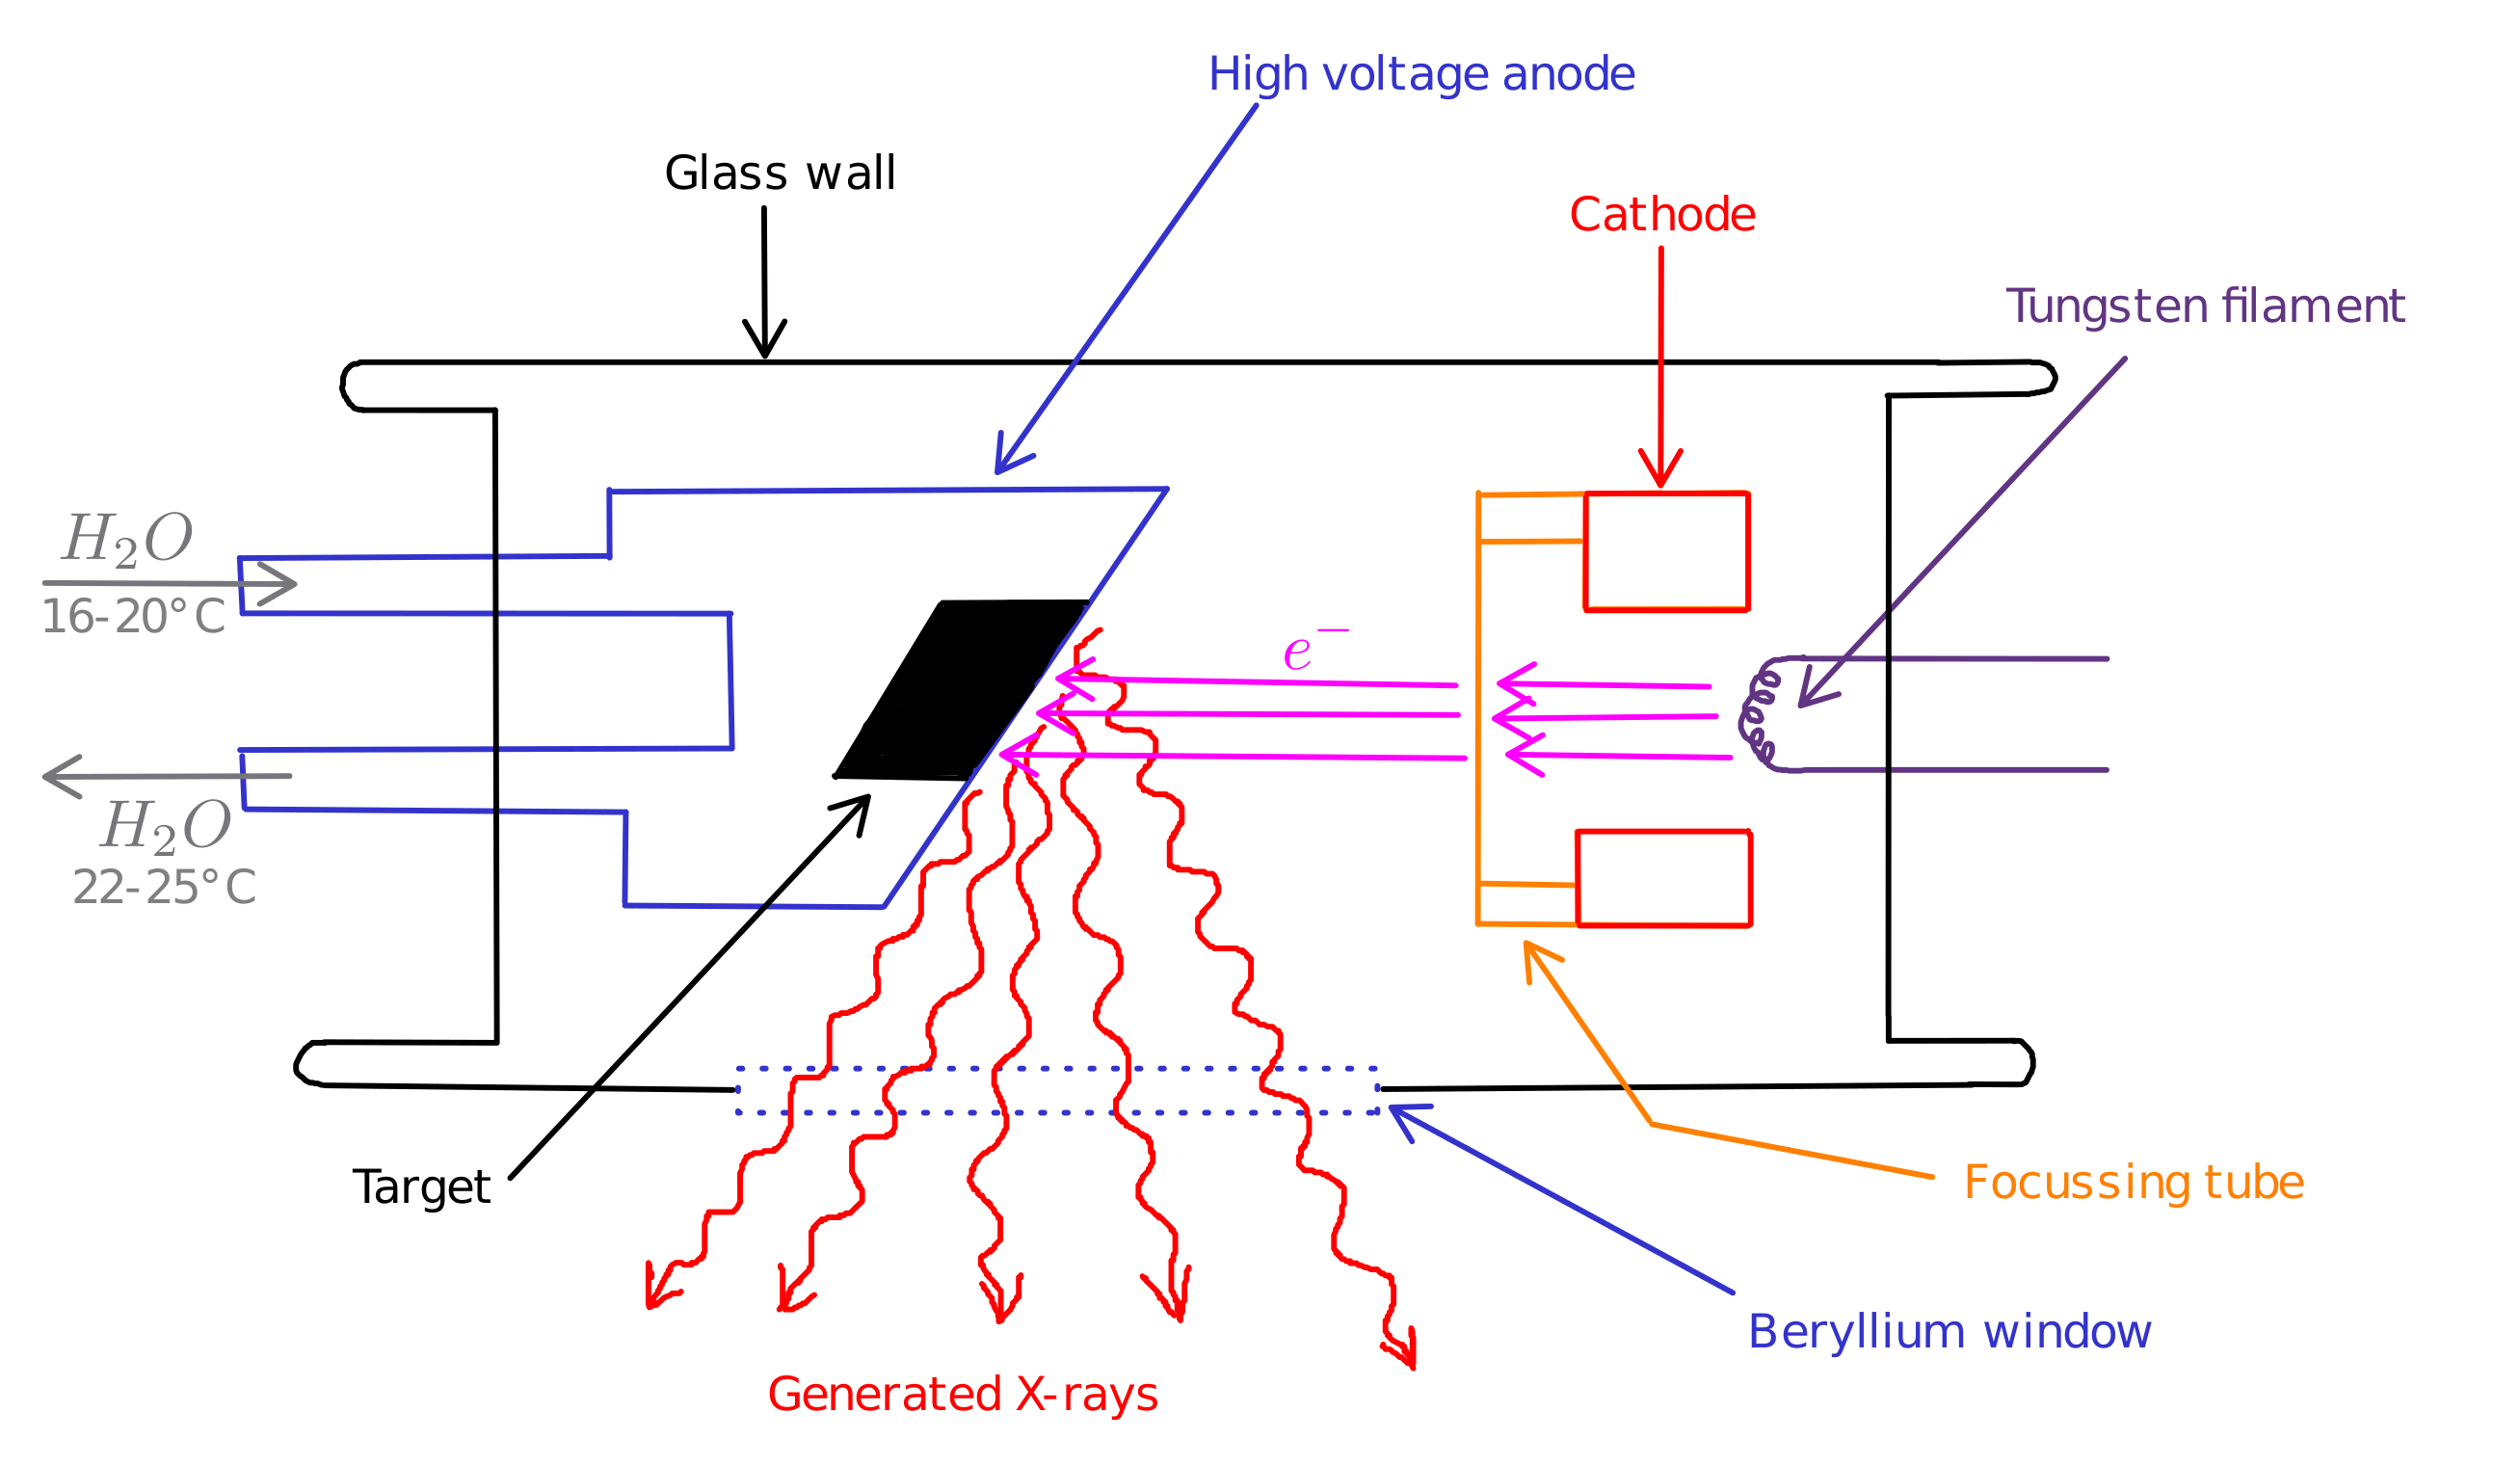
\includegraphics[scale=0.14]{xray_tube.png}
	\caption{\label{fig:xray_tube}Schematic of a X-ray tube.}
\end{figure}

	Figure~\ref{fig:xray_tube} shows the schematic of an X-ray tube. The potential difference between the anode to cathode is around $20-60~\si{kV},$ while the Tungsten filament is supplied a current of $\sim 2-50~\si{mA}.$ The target is composed of the material from which we want to generate the X-rays (generally Cu, Mo or Ag). The Beryllium window provides a transparent region for the generated X-rays to pass through.
	
	The tube is not allowed to cool down between experiments. In the stand-by state, the filament current is reduced to around $\SI{5}{mA}$ and the anode potential is also reduced to $\SI{20}{kV}.$ When data collection is started, the anode voltage is increased to $>\SI{50}{kV}$ and the current in the Tungsten filament is increased to $\SI{40}{mA}.$ In this state, the heated Tungsten filament generates electrons, which are then accelerated and finally hit the target at the anode.

\begin{figure}[h]
	\centering
	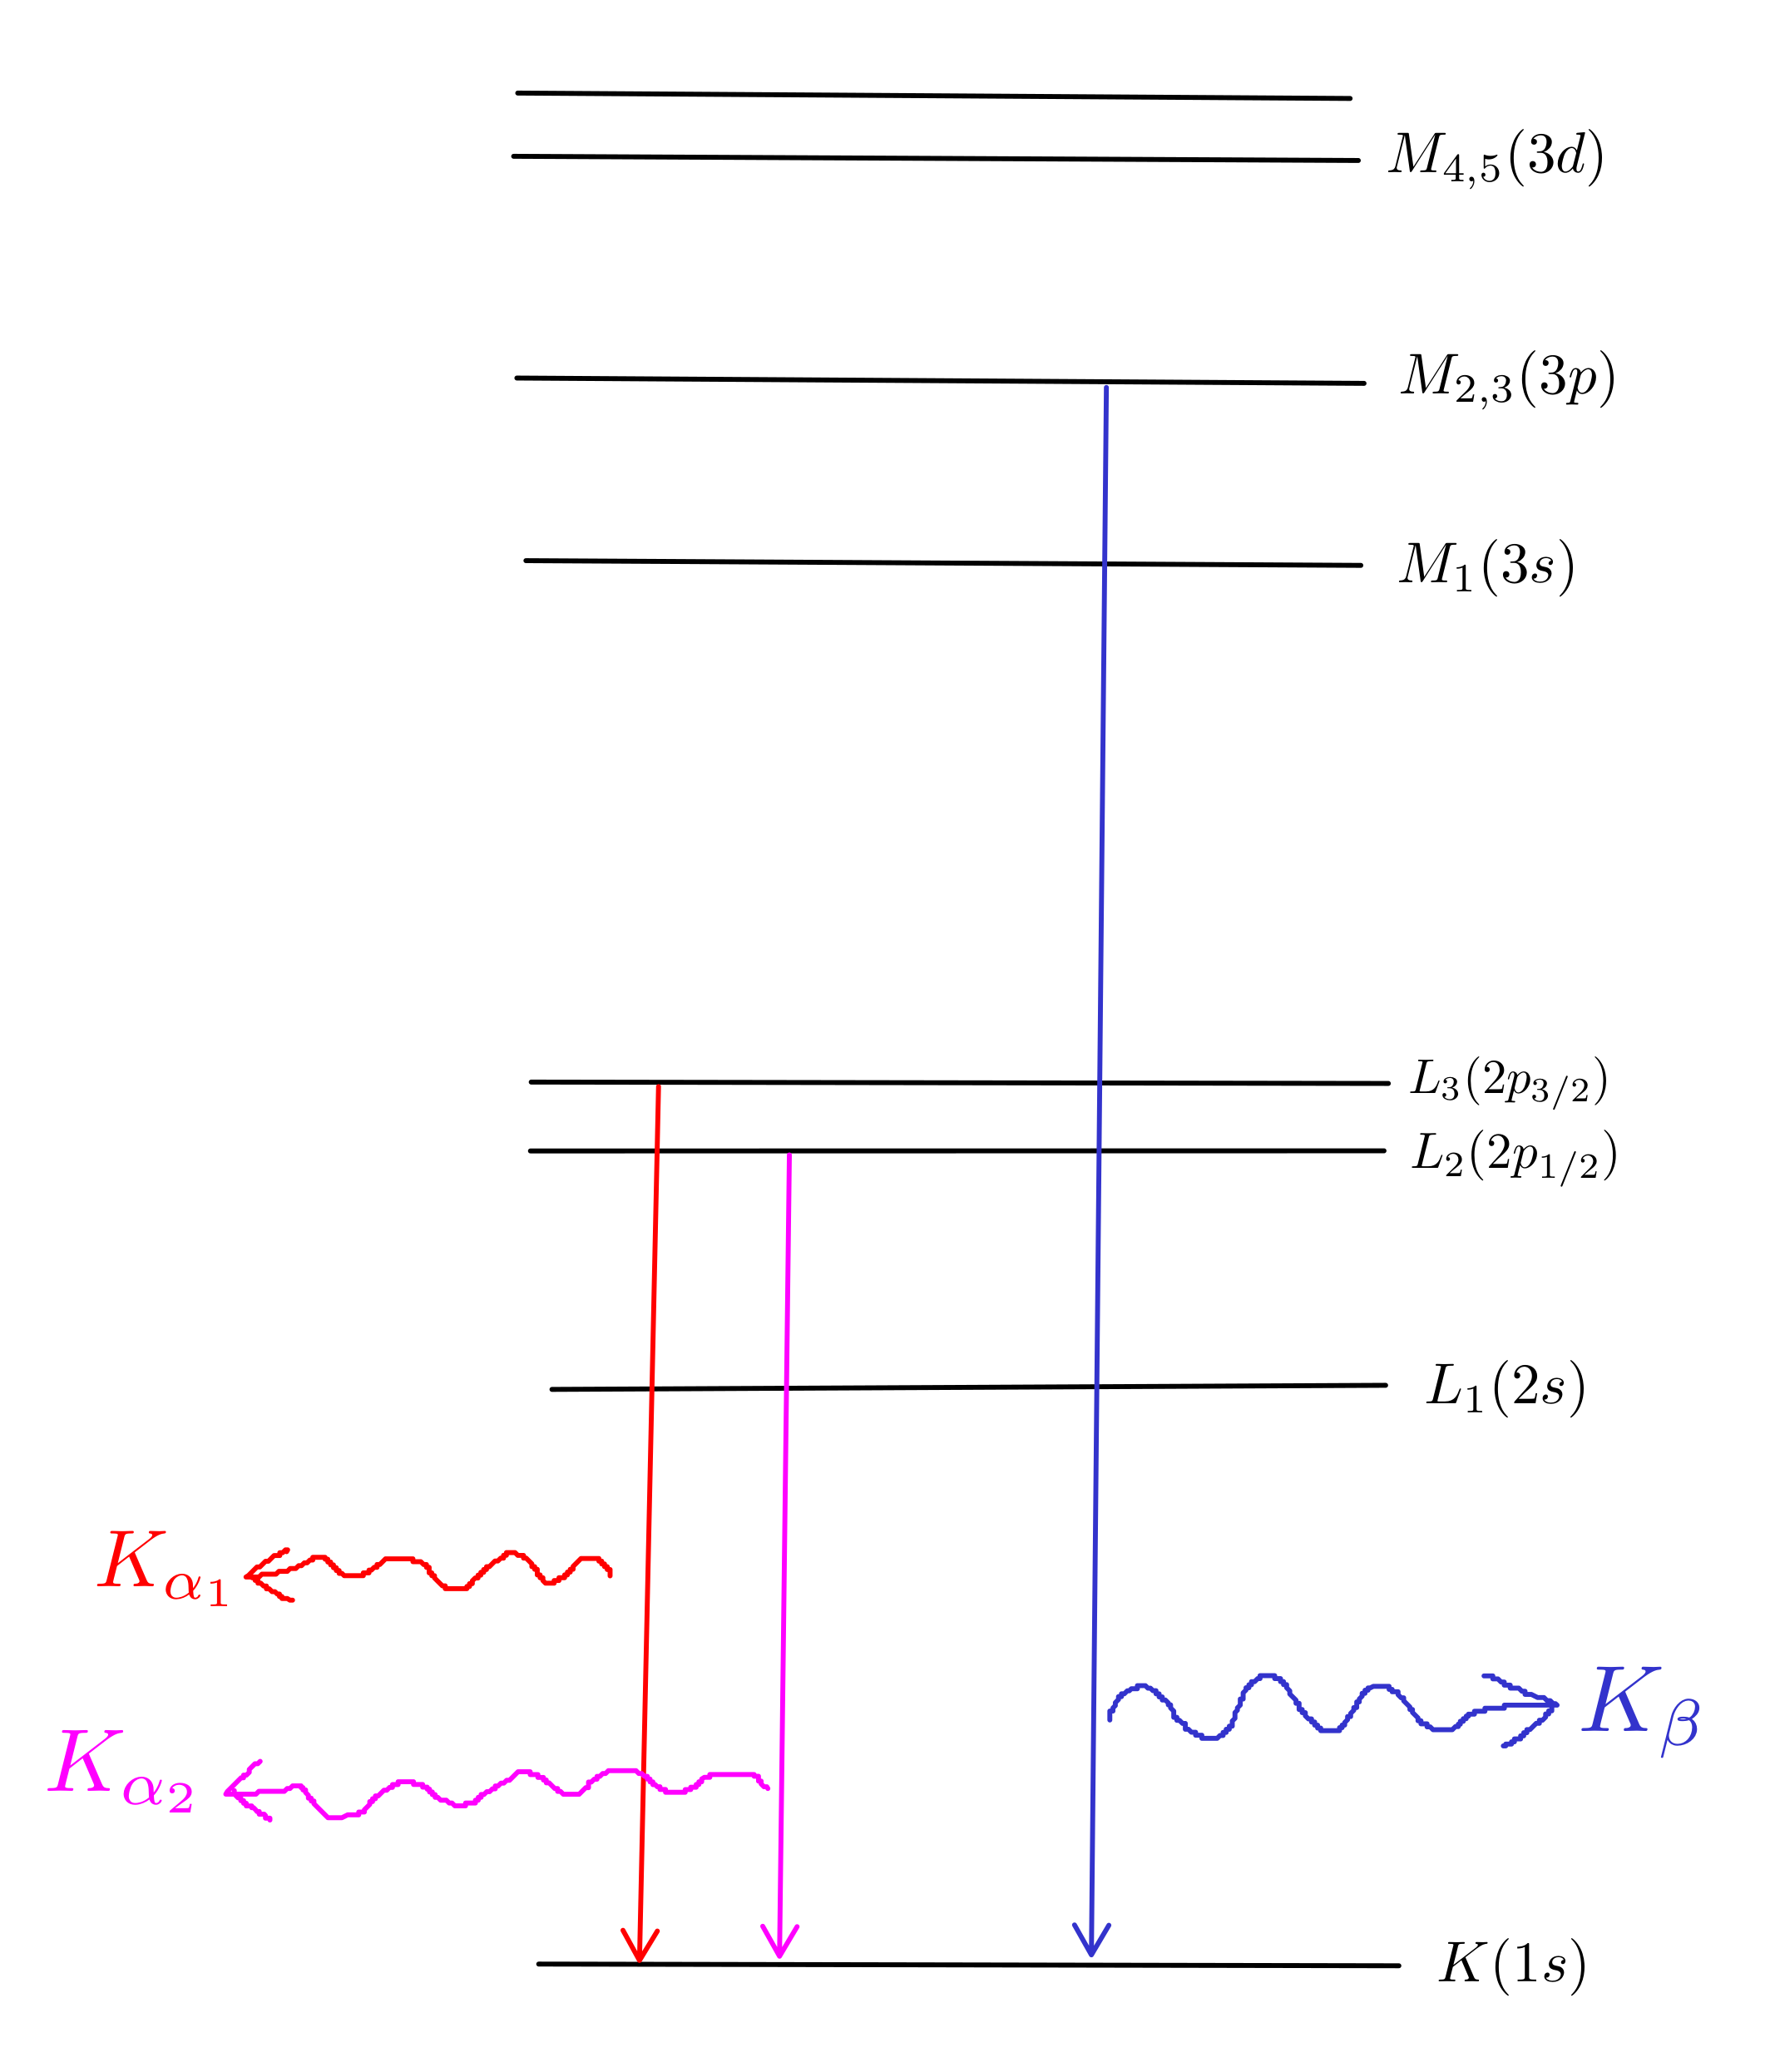
\includegraphics[scale=0.1]{characteristic_xray_transitions.png}
	\caption{\label{fig:xray_transitions}Transitions giving rise to characteristic X-rays.}
\end{figure}
	
	These electrons are able to knock out electrons from the K-shell of an atom in the target. Once an electron is removed from the K-shell, electrons from higher energy levels release energy and come to the K-shell. This release energy is the characteristic X-rays of the material. There are three possible transitions which give rise to X-rays of three different wavelengths. These are shown in figure~\ref{fig:xray_transitions}.
	
\begin{figure}[h]
	\centering
	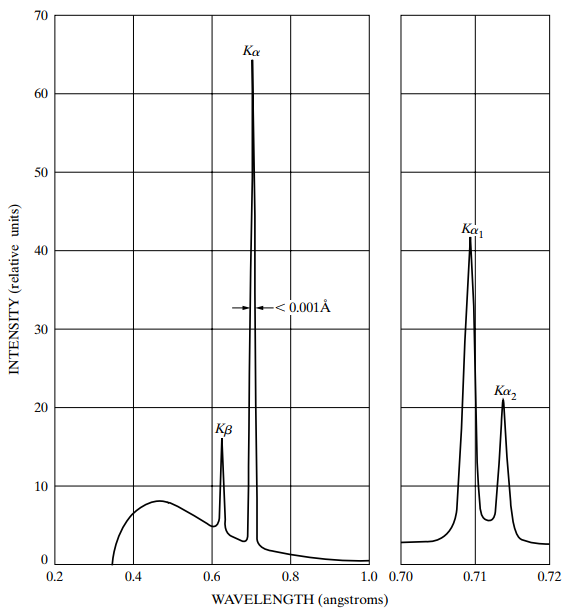
\includegraphics[scale=0.6]{xray_peaks.png}
	\caption{\label{fig:xray_spctra_Cu_Mo}X-ray spectra of $\mathrm{Mo}$ at $\SI{35}{kV}$. The $K_\alpha$ is shown expanded on the right. Picture courtesy:~\cite{Cullity2014}.}
\end{figure}
	
	The X-ray spectra of Mo is shown in figure~\ref{fig:xray_spctra_Cu_Mo}. The $K_\alpha$ peaks are very close to each other. The wavelengths can be found in table~\ref{tab:wavelengths}. The background radiation or white X-rays is attributed to Bremsstrahlung, which is the radiation emitted by electrons when they are decelerated in the X-ray tube.
	
\begin{table}
	\centering
	\caption{\label{tab:wavelengths}Wavelengths of characteristic radiations of Cu and Mo.}
	\begin{tabular}{|c|C|C|C|C|C|c|}
	
		\hline
		
		Source & K_{\alpha_1} (\si{\angstrom}) & K_{\alpha_2} (\si{\angstrom}) & \multicolumn{1}{c|}{\makecell{$K_\alpha$ (average)\\($\si{\angstrom}$)}} & K_\beta (\si{\angstrom}) & Z & $\beta$ filter\\
		
		\hhline{|=|=|=|=|=|=|=|}
		
		Cu & 1.5405 & 1.5433 & 1.5418 & 1.3922 & 29 & Ni (Z = 28) \\
		
		\hline
		
		Mo & 0.7093 & 0.7136 & 0.7107 & 0.6393 & 42 & Nb (Z = 41)\\
		
		\hline
	
	\end{tabular}
\end{table}
	
	We use monochromatic radiation for X-ray diffraction experiments. For this, we have to filter out the unwanted $K_\beta$ and $K_{\alpha2}$ radiations. To filter the $K_\beta$ spectra, we use a $\beta$-filter. The  $\beta$-filters used for Cu and Mo are listed in table~\ref{tab:wavelengths}.
	
	To separate $K_{\alpha1}$ from $K_{\alpha2}$, we use a crystal monochromator. For this, a $\mathrm{Ge}$ crystal is cut along the $(111)$ plane, and the beam with mixed radiation is shined on this plane. Since the two radiations have different wavelengths, they will diffract at two different angles. We can eliminate the unwanted $K_{\alpha2}$ in this way. However, note that \ifnt{the intensity of the reflected beam will fall severely} due to loss of intensity upon reflection.
	
	\section{The physics behind X-ray diffraction}
	
	\section{Type of X-ray diffraction experiments}
	
	\subsection{\label{subsec:crystal_selection}Selection of crystals}

The criteria for selection of crystals for SCXRD is as follows:%
%			
	\begin{itemize}%
%			
	    \item \bfnt{Uniform internal structure}: The crystal should not have more than one domain of array of unit cells, should not be composed of a number of micron or sub-micron sized particles, and should not have crack or distortion of any means. However, \ifnt{the crystal need not have well-defined faces}.
	    
	    \item \bfnt{Suitable size and shape}: For SCXRD experiments, chosen crystals should have dimensions in the range $50-500~\si{\micro\metre}.$ The size of the crystal must be smaller than the spot size of the X-ray beam.
	    
	    \begin{figure}
	    	\centering
	    	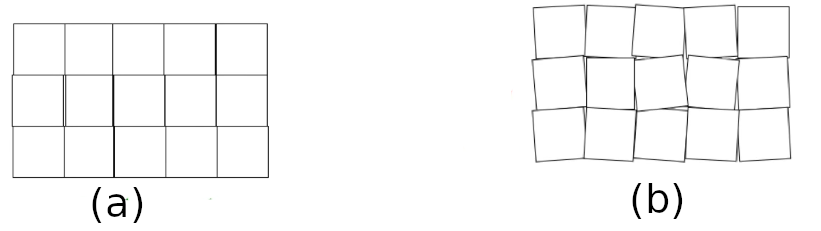
\includegraphics[scale=0.5]{imperfect_crystal.png}
	    	\caption{\label{fig:imperfect_crystal}The crystal on the left is a perfect crystal. The one on the right is a mosaic crystal with a deviation of $\sim 0.1-0.2 \si{\degree}.$ Image courtesy:~\cite{Chowdhury2022}.}
	    \end{figure}
	    
	    \item \bfnt{Imperfect crystals are better.} In perfect crystals, lattice planes traverse in the whole crystal without any deviation, resulting into extinction. Majority of crystals are imperfect, and they diffract better than perfect crystals. Imperfectness may be deliberately introduced into a crystal by a shock.
	    
	    \begin{figure}
	    	\centering
	    	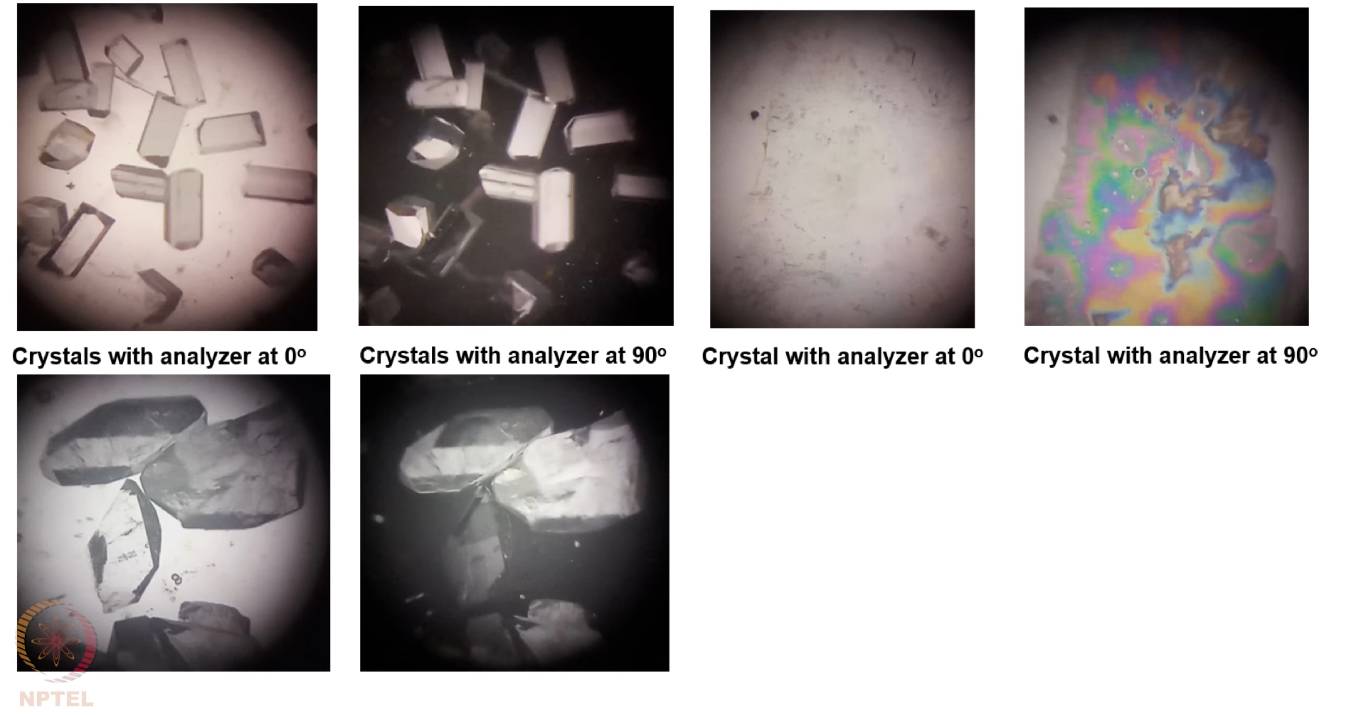
\includegraphics[scale=0.4]{crystal_optical_microscope.png}
	    	\caption{\label{fig:crystal_optical_micro}Crystals when viewed through an optical microscope in polarized light. The set of crystals on the left are good crystals because they are either uniformly dark or uniformly bright when the analyzer is rotated by $\pi/2.$ The crystal on the right shows different colours when the analyzer is rotated, implying that it has more than one domain and cannot be studied under SCXRD. Image courtesy:~\cite{Chowdhury2022}.}
	    \end{figure}
	    
	    \item \bfnt{Screening under optical microscope for domains}: Polarized light is passed through a crystal, and the crystal is rotated about its axis. The transmitted light is observed through an analyser. If, on rotating the analyser, the crystals appears either uniformly dark or uniformly bright in all regions of the crystal, then the crystal has a single domain. Crystals with multiple domains would appear both dark and bright, or show multiple colours at certain angles between the polariser and analyser. This is demonstrated in figure~\ref{fig:crystal_optical_micro}.
	    
	\end{itemize}
	
		We cannot know whether a crystal is good or bad until we mount it on the diffractometer and put it in the path of X-rays. Therefore, when a crystal passes the above minimum selection criteria, we mount it on the goniometer head and shine X-rays on it. The axis about which the crystal is mounted is known as the $\phi$ axis. We rotate crystal about the $\phi$ axis through a full $2\pi$ rotation while keeping the X-ray on for 1-2 minutes depending on the size of the crystal, and we keep recording the diffraction pattern. The diffraction pattern thus recorded is known as the \bfnt{rotation photograph} of the single crystal.
	
	\begin{figure*}
	\centering
	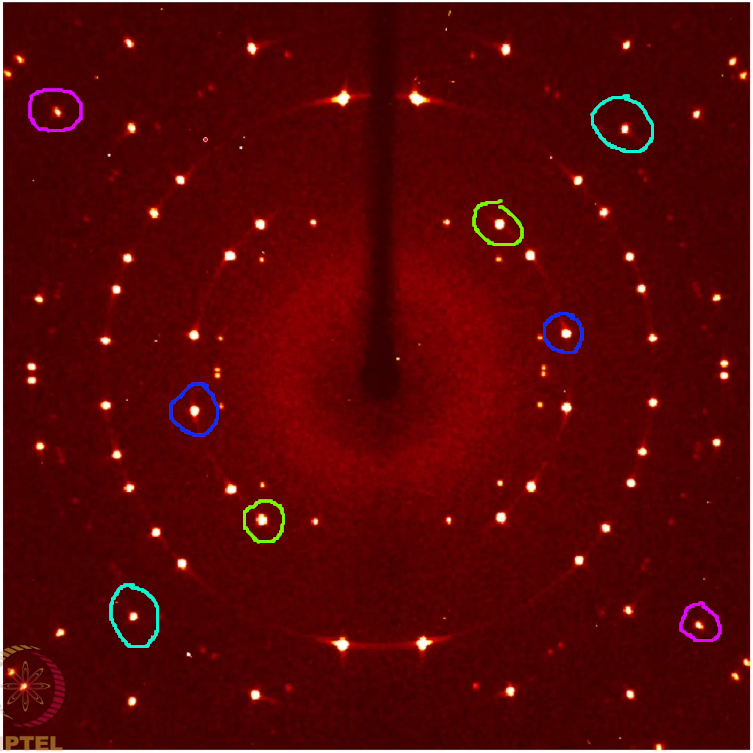
\includegraphics[scale=0.3]{rotation_photograph_mod.png}
	\caption{\label{fig:rotation_photo}Rotation photograph of a single crystal of $\mathrm{NaCl}$. Each spot has another spot on the other side related by a centre of inversion. Some examples are shown by different coloured circles; two spots encircled by the same colour are related to each other. The dark shadow is that of the beam stop, which prevents the direct X-ray beam from falling on the detector. Image courtesy:~\cite{Chowdhury2022}.}
	\end{figure*}
	
	Figure~\ref{fig:rotation_photo} shows the rotation photograph of a single crystal. This photograph is always centrosymmetric irrespective of the type of crystal geometry. Each spot on the rotation photograph has another corresponding spot that is related to it by a centre of inversion. If instead of these spots, the rotation photograph is composed of concentric circles, we conclude that the crystal is not a single crystal, but a polycrystal, and is not suitable for XRD.
	
	\section{Mounting a crystal on SCXRD diffractometer}

	\begin{figure*}[t]
		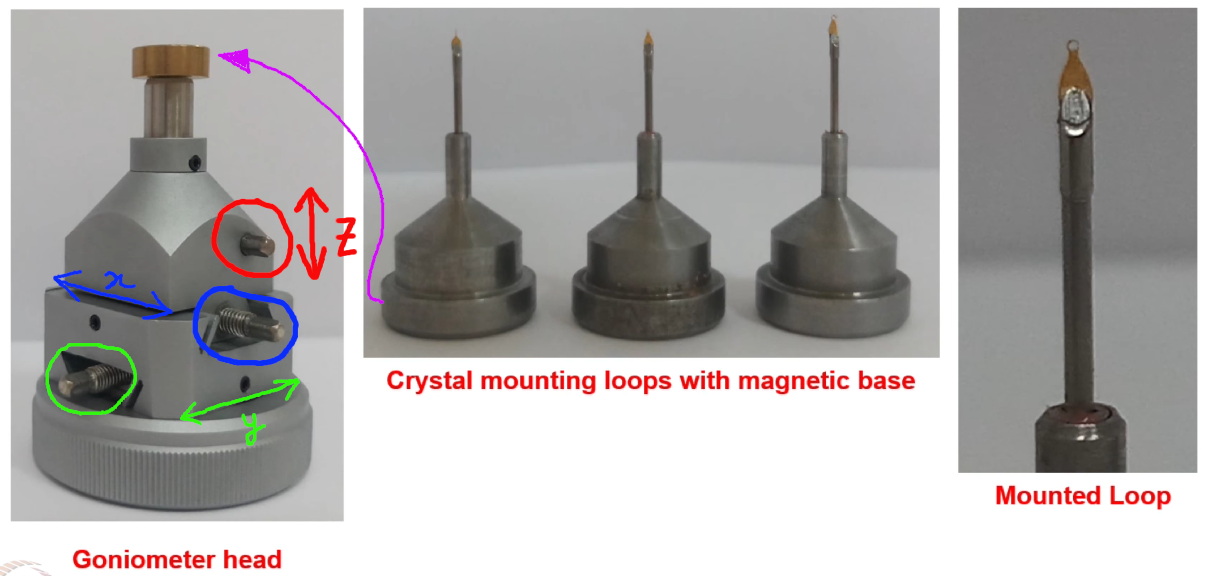
\includegraphics[scale=0.5]{goniometer_mod.png}
		\caption{\label{fig:goniometer}The goniometer head, mounting loop with the mounting base.}
	\end{figure*}

	In fig.~\ref{fig:goniometer}, a goniometer head is shown. This head is mounted on the goniometer of the diffractometer. The top of the goniometer head is a magnetic base which allows the mounting loops to be held in place. To align the crystal in the X-ray beam, the goniometer head has three screws that allow movement in the three Cartesian directions. These screws and their respective directions have been demarcated in the figure.

		The tip of the mounting metal pin has a small polymer loop. The crystal is mounted on this loop using some thick oil, which keeps the crystal in place by its surface tension. These loops are available in various diameters, generally in the range $0.05-0.5~\si{mm}.$

		Nylon loops are also available, in which the loop is made by a nylon thread, which is then twisted several times and then glued to a pin. The pin is attached to a brush, which can be directly mounted on the goniometer head and placed in the X-ray beam.

	\section{The SCXRD diffractometer and its types}
	
	\section{How much data do we have to collect?}
	
	
		

\end{document}